\documentclass[11pt]{article}
\usepackage[utf8]{inputenc}
\usepackage{amsmath}
\usepackage{float}
\usepackage[T1]{fontenc}
\usepackage{lmodern}
\usepackage{geometry}
\usepackage{graphicx}
\usepackage{booktabs}
\usepackage{array}
\usepackage{tabularx}
\usepackage{enumitem}
\usepackage{xcolor}
\usepackage{tikz}
\usetikzlibrary{positioning,arrows.meta,fit,backgrounds}
\usepackage{hyperref}
\geometry{a4paper, margin=1in}
\hypersetup{colorlinks=true, linkcolor=black, urlcolor=blue!50!black, citecolor=black}
\setlist{itemsep=2pt, topsep=4pt}
\renewcommand{\arraystretch}{1.25}
\setlength{\emergencystretch}{2em}
\newcolumntype{L}{>{\raggedright\arraybackslash}X}

\title{\textbf{Secure Multi-Tenant Identity and Access Platform\\[2pt]\large Final Project Report}}
\author{Team P01-G33\\[4pt]
Krishna Teja (CS23BTECH11028) \and Jaya Prakash (CS23BTECH11015)\\[4pt]
Department of Computer Science and Engineering\\
Indian Institute of Technology Hyderabad}
\date{November 2026}

\begin{document}
\maketitle

\begin{center}
Repository: \url{https://github.com/krishnateja2314/iam-provider}
\end{center}

\begin{abstract}
We built a working multi-tenant identity and authorization platform for a learning SaaS. From a clean clone with new volumes, 227 of 227 automated security tests pass against it (0 failed, 0 skipped), including 16 cases against a live identity provider.
The platform lets one person belong to several organizations with a different role in each, and guarantees that a role in one organization never leaks into another. Authentication is delegated to Keycloak 26.8.0 using the OAuth~2.0 authorization-code flow with S256 PKCE. Everything identity providers usually leave to the application is ours: global user mapping, tenant memberships, resource ownership, Casbin-based authorization with deny-overrides, idempotent tenant provisioning, purpose-specific consent and transactional audit logging.
A reporting agent runs as an application service principal with exactly one action in one tenant, and its audit rows identify it as a service.
The backend is a modular monolith (Node.js 24, Fastify 5, PostgreSQL 16), started with one Docker Compose command. Beyond the test suite, a Playwright script proves real browser PKCE and enterprise-federation logins, revoked sessions are denied on the very next request (26--146\,ms after the call), and a mutation script shows that the tests catch each of 11 deliberately broken security guards. User-delegated agents, full SCIM and native mobile apps are documented as future work rather than claimed.
\end{abstract}

\section{Introduction and motivation}
A learning SaaS serves people who arrive through different doors: a student signing in from a phone, an instructor publishing from a laptop, and an enterprise employee enrolled by their company. The same person can also belong to several organizations at once. Our running example is Sam, who is an \textbf{administrator in Amaravati Learning} and simultaneously \textbf{a learner in IITH University}. Sam's admin rights at Amaravati must never apply inside IITH.

When identity logic is baked into the main application, this breaks quickly. Every new service re-implements its own permission checks, tenant IDs passed by the client get trusted by mistake, and audit questions turn into manual investigations. The standard answer is to separate identity and access management into its own layer that the rest of the system can trust.

\subsection*{Problem statement}
Design and implement an identity and access platform that cleanly separates four concerns: \textbf{authentication} (who is this), \textbf{user profile} (what do we know about them), \textbf{tenant membership} (which organizations, in which role) and \textbf{authorization} (may they do this specific thing right now). It must support consumer and enterprise sign-in, a secure session lifecycle, fine-grained authorization, tenant provisioning, consent and auditing, and it must prove through automated adversarial tests that tenant and privilege boundaries hold.

\subsection*{Five shortcuts we set out to avoid}
\begin{enumerate}
  \item Trusting the organization ID that the client sends.
  \item Putting tenant roles inside the login token, where they stay valid until expiry.
  \item Merging accounts because two email addresses match.
  \item Trusting a token until it expires, so logout does not really log anyone out.
  \item Treating audit logging as an afterthought.
\end{enumerate}

\subsection*{Milestones}
The project brief defined seven milestones, which structure the rest of this report.

\begin{table}[H]
\centering
\begin{tabularx}{\textwidth}{@{}l l L@{}}
\toprule
\textbf{ID} & \textbf{Milestone} & \textbf{What must be demonstrable}\\
\midrule
M1 & Identity and tenant model & Users, external identities, profiles, organizations, memberships and roles are separate linked entities\\
M2 & Sign-in and federation & Two authentication mechanisms on web and mobile, one of them enterprise federation\\
M3 & Session lifecycle & Token expiry, refresh rotation, logout, revocation and replay rejection follow a written policy\\
M4 & Fine-grained authorization & A declarative policy engine evaluated over at least 40 access scenarios\\
M5 & Tenant provisioning & Idempotent organization creation, admin bootstrap, quotas, suspend and reactivate\\
M6 & Consent and audit & Queryable audit records; downstream views expose only permitted profile fields\\
M7 & Security validation & Automated tests prove cross-tenant access, escalation, revoked sessions and malformed claims are denied\\
\bottomrule
\end{tabularx}
\caption{Project milestones.}
\end{table}

\section{Background and related work}
Mature identity providers already exist, so our contribution is not a new login server but the application-side layer that those products leave to each customer. Commercial products (Okta, Microsoft Entra ID, Auth0, AWS Cognito) and open-source ones (Keycloak, Ory, Zitadel) all implement OpenID Connect and OAuth~2.0 well. Most of them treat authorization as coarse roles and groups, and push fine-grained, tenant-aware decisions back into the application.

Authorization itself is fragmented. RBAC is built into most frameworks, ABAC is expressed in standards like XACML or policy-as-code engines like OPA, and relationship-based access control (ReBAC) comes from Google's Zanzibar via SpiceDB and OpenFGA. Real systems mix all three, which is what milestone M4 asks for.

The brief named five references. Each shaped a concrete design decision.

\begin{table}[H]
\centering
\begin{tabularx}{\textwidth}{@{}p{4.2cm} L l@{}}
\toprule
\textbf{Reference} & \textbf{What we took from it} & \textbf{Milestones}\\
\midrule
OpenID Connect Core 1.0 \cite{oidc} & Authorization-code flow; ID token for the client, access token for the API; nonce and state checks & M2, M3\\
OAuth 2.0 Security BCP, RFC 9700 \cite{bcp} & PKCE for public clients, no implicit or password grants, refresh-token rotation and reuse detection & M3, M7\\
Zanzibar (USENIX ATC 2019) \cite{zanzibar} & Treat ``instructor teaches course'' as a relationship fact checked at decision time, at small scale & M4\\
SCIM, RFC 7644 \cite{scim} & Idempotent, transactional organization provisioning as the minimal enterprise slice & M5\\
NIST Privacy Framework \cite{nist} & Purpose-specific consent, data minimization through field allowlists, queryable audit & M6\\
\bottomrule
\end{tabularx}
\caption{Reference works and how they shaped the design.}
\end{table}

The gap we target is a small, testable reference implementation that separates authentication from tenant authorization end to end, combines role, attribute and relationship rules in one decision path, and backs every security claim with an executed test.

\section{Proposed approach and system architecture}
Our approach is reuse-first: Keycloak proves who someone is, and our own backend decides what that person or program may do right now in a specific organization. Five design decisions follow from that split.

\paragraph{1. Modular monolith instead of microservices.}
Our Week~0 proposal listed eight services. Mentor review pointed out that eight deployments would eat the eight-week schedule in networking and distributed-transaction work. We kept the eight logical modules but run them in one Fastify process sharing one PostgreSQL database, which also gives us ACID transactions for ``mutation plus audit'' atomicity.

\begin{table}[H]
\centering
\begin{tabular}{@{}lccc@{}}
\toprule
\textbf{Criterion} & \textbf{Microservices} & \textbf{\shortstack{Traditional\\monolith}} & \textbf{\shortstack{Modular monolith\\(chosen)}}\\
\midrule
Development effort & High & Low & Medium\\
Module separation & Strong & Weak & Strong\\
Deployment effort & High & Low & Low\\
Eight-week risk & High & Low & Low to medium\\
Future extraction into services & Natural & Hard & Natural\\
\bottomrule
\end{tabular}
\caption{Architecture options considered after the Week 0 review.}
\end{table}

\paragraph{2. Keycloak for authentication, not a custom OIDC server.}
Writing a secure authorization server is a separate security project. Keycloak 26.8.0 handles credential storage, login pages, RS256 token signing, refresh rotation and enterprise federation. Our clients never see a password.

\paragraph{3. Casbin for authorization, with facts in our database.}
We evaluated Keycloak's built-in authorization services and found them awkward for tenant-specific and relationship rules. Putting tenant roles in token claims would also leave them stale until the token expires. Instead, memberships, roles, teaching assignments and policy rows live in PostgreSQL, and Casbin 5.51.1 evaluates them fresh on every decision with a deny-overrides effect:
\[
\textit{allowed} \;=\; \exists\,\text{allow} \;\wedge\; \neg\exists\,\text{deny}.
\]

\paragraph{4. Identity keyed by issuer and subject, never by email.}
Many apps merge accounts when emails match, which enables account takeover through recycled or unverified emails. We key every external identity by \texttt{(issuer, subject)} and never merge on email.

\paragraph{5. Programs are not users.}
A reporting agent calls the API with the OAuth client-credentials grant. Treating it as a user would create a fake account with a membership whose roles could later widen what the agent can do. Instead it is a separate principal kind with its own registry and an explicit list of \texttt{(tenant, resource, action)} grants, and it never receives a membership or a role (Section~\ref{sec:ag01}).

\subsection{Architecture}
Docker Compose runs five containers: the web/mobile client server, Keycloak, Keycloak's private database, the Fastify backend and the application database. Both databases have no host ports. The protected request path is a fixed pipeline of hooks, so no route can skip tenant checks (Figure~\ref{fig:arch}).

\begin{figure}[H]
\centering
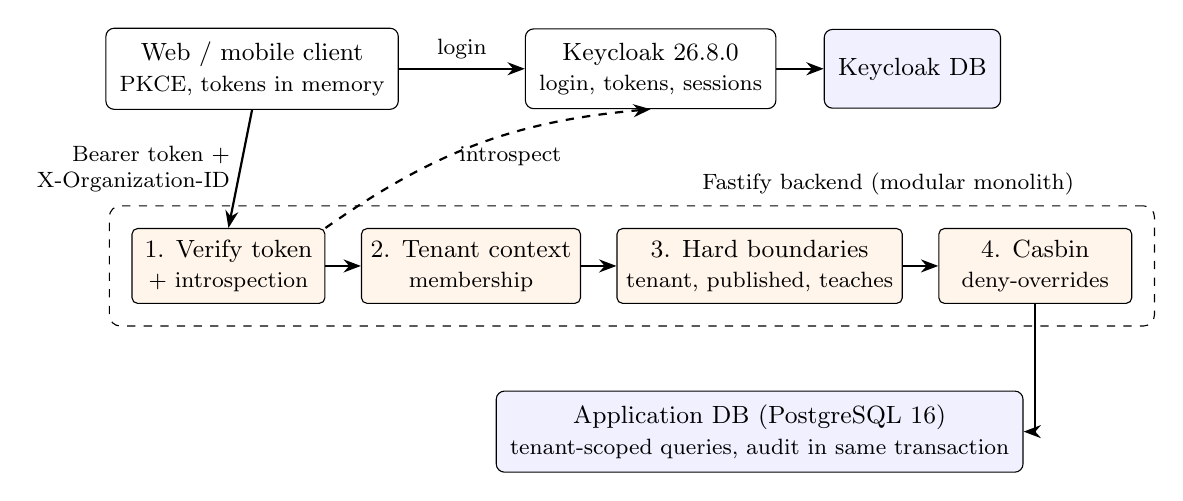
\begin{tikzpicture}[
  font=\small,
  box/.style={draw, rounded corners=3pt, align=center, minimum height=1.0cm, inner sep=5pt, fill=white},
  stage/.style={draw, rounded corners=2pt, align=center, minimum width=2.45cm, minimum height=0.95cm, fill=orange!8},
  db/.style={draw, rounded corners=3pt, align=center, minimum height=1.0cm, inner sep=5pt, fill=blue!6},
  arr/.style={-{Stealth[length=2.2mm]}, thick},
  node distance=0.55cm and 0.45cm]
\node[box] (client) {Web / mobile client\\\footnotesize PKCE, tokens in memory};
\node[box, right=1.6cm of client] (kc) {Keycloak 26.8.0\\\footnotesize login, tokens, sessions};
\node[db, right=0.6cm of kc] (kcdb) {Keycloak DB};
\node[stage, below=1.5cm of client, xshift=-0.3cm] (s1) {1. Verify token\\\footnotesize + introspection};
\node[stage, right=of s1] (s2) {2. Tenant context\\\footnotesize membership};
\node[stage, right=of s2] (s3) {3. Hard boundaries\\\footnotesize tenant, published, teaches};
\node[stage, right=of s3] (s4) {4. Casbin\\\footnotesize deny-overrides};
\begin{scope}[on background layer]
\node[draw, dashed, rounded corners=4pt, fit=(s1)(s4), inner sep=8pt, label={[font=\footnotesize]above right:Fastify backend (modular monolith)}] (api) {};
\end{scope}
\node[db, below=1.1cm of s3] (appdb) {Application DB (PostgreSQL 16)\\\footnotesize tenant-scoped queries, audit in same transaction};
\draw[arr] (client) -- node[above, font=\footnotesize]{login} (kc);
\draw[arr] (kc) -- (kcdb);
\draw[arr] (client.south) -- node[left, font=\footnotesize, align=right]{Bearer token +\\X-Organization-ID} (s1.north);
\draw[arr] (s1) -- (s2); \draw[arr] (s2) -- (s3); \draw[arr] (s3) -- (s4);
\draw[arr, dashed] (s1.north east) to[bend left=15] node[right, font=\footnotesize, pos=0.4]{introspect} (kc.south);
\draw[arr] (s4.south) |- (appdb.east);
\end{tikzpicture}
\caption{System architecture and the protected request pipeline. Failing any stage stops the request with 401, 403 or 404, and nothing reaches the database without an organization filter.}
\label{fig:arch}
\end{figure}

\section{Implementation}
The prototype is about 2,600 lines of backend TypeScript and 2,200 lines of tests, across eight backend modules, two browser clients, two Keycloak realm definitions and ten test files.

\subsection{Technology stack}
\begin{table}[H]
\centering
\begin{tabularx}{\textwidth}{@{}l l L@{}}
\toprule
\textbf{Layer} & \textbf{Tool and version} & \textbf{Role}\\
\midrule
Runtime and API & Node.js 24.21.0, Fastify 5.12.8 & Modular monolith, hooks, schema validation\\
Database & PostgreSQL 16.15, Kysely 0.29.6 & Type-safe queries, migrations, constraints and triggers\\
Identity provider & Keycloak 26.8.0 & OIDC login, token signing, refresh rotation, enterprise broker\\
Authorization & Casbin 5.51.1 & Declarative role/resource/action policy with deny-overrides\\
Token validation & jose 6.2.12 & RS256 signature and claim verification against JWKS\\
Testing & Vitest 5.0.3, Playwright 1.63.0 & Security and integration tests; real browser login proof\\
Infrastructure & Docker Compose & Five services, private database network\\
\bottomrule
\end{tabularx}
\caption{Technology stack.}
\end{table}

\subsection{Backend modules}
\begin{table}[H]
\centering
\begin{tabularx}{\textwidth}{@{}l p{5.6cm} L@{}}
\toprule
\textbf{Module} & \textbf{File} & \textbf{Responsibility}\\
\midrule
Auth & \texttt{\footnotesize token-validator.ts}, \texttt{\footnotesize session-service.ts} & Verify access tokens, introspect sessions, list and revoke sessions\\
User & \texttt{\footnotesize user-service.ts}, \texttt{\footnotesize privacy-service.ts} & Map \texttt{(issuer, subject)} to a global user; consent and profile projection\\
Organization & \texttt{\footnotesize membership-service.ts} & Memberships and current tenant roles\\
Authorization & \texttt{\footnotesize authorization-engine.ts} & Hard boundaries, then Casbin evaluation\\
Learning resource & \texttt{\footnotesize resource-service.ts} & Tenant-bound course and assignment queries\\
Provisioning & \texttt{\footnotesize provisioning-service.ts} & Idempotent organization creation, quotas, suspend and reactivate\\
Audit & \texttt{\footnotesize audit-service.ts} & Insert and query audit events, optionally inside a transaction\\
Service principal & \texttt{\footnotesize service-principal-service.ts} & Agent registry, tenant gate and exact-grant authorization\\
\bottomrule
\end{tabularx}
\caption{Backend modules (files under \texttt{backend/src/modules/}).}
\end{table}

\subsection{How a protected request is handled}
\begin{enumerate}
  \item The client logs in with authorization code plus S256 PKCE, keeps tokens in memory only, and calls the API with the access token as a Bearer token in the \texttt{Authorization} header, plus an \texttt{X-Organization-ID} header.
  \item \texttt{authenticationHook} verifies the RS256 signature against Keycloak's JWKS, plus issuer, audience \texttt{iam-backend}, expiry, subject and \texttt{typ=Bearer}. ID tokens are rejected with 401.
  \item The backend makes an uncached introspection call to Keycloak, so a logged-out or revoked session fails on the next request. If Keycloak is unreachable, the request fails closed.
  \item \texttt{tenantContextHook} treats the organization header as untrusted input and requires an active membership in an active organization, otherwise 403. A service principal instead needs an active organization in which it holds a grant.
  \item \texttt{authorize()}, given the subject, organization, resource, action and context, applies hard boundaries first: published-only resources for non-admins, submission ownership, and the teaching relationship for instructors who read or grade.
  \item Casbin evaluates the user's full current role set. The effect is ``some allow and no deny'', so an explicit deny wins even if another role allows.
  \item Every query filters on both the resource ID and \texttt{organization\_id}, so a guessed ID from another tenant returns 404.
  \item Mutations such as grading write their audit event in the same PostgreSQL transaction. If the audit insert fails, the grade rolls back.
\end{enumerate}

\subsection{Data model and integrity}
User, external identity, profile, organization, membership and role are separate tables, and service principals and their grants have their own two tables (migration 004). Composite foreign keys tie role assignments, teaching assignments and submissions to the same organization, so the database itself rejects a cross-tenant link even if application code had a bug. Quota triggers lock the organization row before counting, which prevents two concurrent requests from both taking the last slot.

\subsection{Weekly progress}
\begin{table}[H]
\centering
\begin{tabularx}{\textwidth}{@{}l p{4.4cm} L@{}}
\toprule
\textbf{Week} & \textbf{Focus} & \textbf{Outcome}\\
\midrule
Week 0 & Problem understanding and related work & Seven milestones, five references mapped, eight-component proposal\\
Week 1 & Detailed design after mentor review & Modular monolith, data model, threat model with 10 invariants, first 15 authorization scenarios\\
Week 2 & Core implementation & Keycloak + Fastify + Casbin running in Compose; 159 tests passing; real browser PKCE proof\\
Week 3 & Mentor feedback (P0/P1) and evidence & Published repository, introspection safe by default, centralized tenant guards, test-independence script, evaluation protocol frozen (one day late)\\
Week 4 & Week 3 review (P1) & Suspended consent withdrawal restored, fatal startup check, exact 503 outage contract, per-tenant domain/SSO association, real adversarial fixtures, reliable mutation runner, configurable public host; 197 tests from a clean clone\\
Week 5 & Plan from the Week 4 report & Dependency advisories fixed (\texttt{npm audit}: 0); AG01 application service principal; four new mutations; latency observation; 227 tests from a clean clone\\
\bottomrule
\end{tabularx}
\caption{Weekly progress.}
\end{table}

\subsection{Responding to mentor feedback}
The Week~2 review raised priority items, all of which we closed. The repository returned 404 for the mentor, so we published it. Introspection could be switched off by a flag, so we made it default to on and fatal to disable when \texttt{NODE\_ENV=production}. We added tests for an unseeded third organization and for header/resource-ID substitution, and wrote a script that proves our tests catch deliberately broken guards.

The Week~3 review found that some of that evidence was weaker than claimed. Rerunning the code on a real database confirmed a regression: the stricter tenant guard blocked suspended members from withdrawing consent. The old mutation script reported success on any error, including a stopped database, and one adversarial test used an ID that could never match. In Week~4 we fixed each item and rebuilt the evidence from a clean clone. The mutation runner now reports infrastructure failures as inconclusive (exit code 2). The adversarial tests use a real foreign submission and a third tenant provisioned over HTTP. We also corrected two of our own earlier answers that had overstated what was run. No review of the Week~4 report had been received at the time of writing, so Week~5 carried out the plan that report committed to.

\section{Experimental results and evaluation}
All results in this section come from one run on 7 November 2026: a fresh \texttt{git clone} of revision \texttt{fde2efd}, started with new Docker volumes so the realm import, migrations and seed ran from scratch (Node 24.21.0, PostgreSQL 16.15, Keycloak 26.8.0, Vitest 5.0.3, Windows 11 with Docker Desktop). The complete suite passed \textbf{227 of 227 tests, with 0 failures and 0 skipped}. Typecheck of source and tests and the production build passed. \texttt{npm audit} reported 0 vulnerabilities, after we fixed the four advisories that had appeared in Week~4 and a new one in a test dependency. Raw logs are in \texttt{docs/evidence/2026-11-07/}.

\begin{table}[H]
\centering
\begin{tabularx}{\textwidth}{@{}p{4.6cm} L r@{}}
\toprule
\textbf{Test suite} & \textbf{What it attacks or checks} & \textbf{Passed}\\
\midrule
\texttt{\footnotesize t05-t08-authorization} & 48 role/resource/action cases plus 11 hard-boundary, role-change and deny-precedence cases & 59\\
\texttt{\footnotesize t03-t04-t09-token-validation} & Wrong key, issuer, audience, algorithm; expired tokens; ID token used as API credential; malformed claims & 41\\
\texttt{\footnotesize api} (integration) & Real foreign submission and third tenant, non-member headers, unrelated grading, audit-failure rollback, consent under suspension, exact 503 on provider outage & 31\\
\texttt{\footnotesize service-principal} (7 live) & AG01 agent: one grant, other tenants and admin actions denied, expiry, disablement, audit, introspection binding & 30\\
\texttt{\footnotesize session-lifecycle} (6 live) & Introspection contract; live logout, revocation, logout-all, password reset, refresh expiry and replay & 21\\
\texttt{\footnotesize startup-config} & Unsafe configuration stops the server before it binds a port (subprocess) & 12\\
\texttt{\footnotesize tenant-sso} (3 live) & Per-tenant email domain and broker association; live Keycloak routing & 10\\
\texttt{\footnotesize provisioning-privacy} & Concurrent idempotent provisioning, payload conflicts, quotas, suspend and reactivate, consent & 9\\
\texttt{\footnotesize t01-t02-identity-membership} & Issuer/subject uniqueness, no email merge, 12 concurrent first logins create one user & 8\\
\texttt{\footnotesize t10-audit} & Required audit fields, filtering, no secrets logged & 6\\
\midrule
\textbf{Total} & & \textbf{227}\\
\bottomrule
\end{tabularx}
\caption{Test suites and results.}
\end{table}

\subsection{Session revocation latency}
We measured the time from a logout or revocation call until the next API request with the old token was denied. Every case returned 401 on the first request after the operation, without retries.

\begin{table}[H]
\centering
\begin{tabular}{@{}lcc@{}}
\toprule
\textbf{Operation} & \textbf{First request} & \textbf{Operation to denial}\\
\midrule
Provider logout & 401 & 45\,ms\\
Own-session revocation via API & 401 & 41\,ms\\
Admin logout-all & 401 & 26\,ms and 146\,ms\\
Agent client disabled in Keycloak (AG01) & 401 & 23\,ms\\
\bottomrule
\end{tabular}
\caption{Revocation latency (local samples from the clean run).}
\end{table}

These are local samples (maximum 146\,ms, against a 5-second test bound), not a service-level guarantee. The Week~4 run observed 31--158\,ms.

\subsection{AG01: the reporting agent as a service principal}
\label{sec:ag01}
The Week~4 report committed to one executable agent outcome with fixed expected results. The Keycloak client \texttt{iam-agent-reporting} may use only the client-credentials grant. Its tokens carry audience \texttt{iam-backend}, no realm roles, no user session and a provider-stamped \texttt{principal\_kind=service}. Introspection must report the token active, issued to that client and bound to that client's own service account. The backend then looks the client up in a \texttt{service\_principals} registry and allows only the actions listed in \texttt{service\_principal\_grants}. The seed grants exactly one: list learning resources in Acme. Identity, session, consent and platform routes refuse service principals. A service token never creates a user, identity or membership row.

\begin{table}[H]
\centering
\begin{tabularx}{\textwidth}{@{}L L@{}}
\toprule
\textbf{Expected (Week 4 plan)} & \textbf{Observed with real Keycloak tokens}\\
\midrule
Acme resource list: 200 & 200; every row belongs to Acme and is published\\
Globex: 403 & 403 (no grant in Globex)\\
An admin action in Acme: 403 & 403 for members, audit, SSO config and single-resource read; \texttt{/me} also 403\\
Expired token: 401 & 401 (a 2-second token, used after 3.5 seconds)\\
Already-issued token after the client is disabled: 401 & 401 on the first request, 23\,ms after the change; a new token request fails with \texttt{invalid\_client}\\
Audit rows with \texttt{actor\_type='service'} & Allow and deny rows name the service principal as actor and record the client ID\\
\bottomrule
\end{tabularx}
\caption{AG01 outcomes (\texttt{service-principal.test.ts}, 7 live cases; 23 more fixture and introspection cases).}
\end{table}

One provider behaviour surprised us. Re-enabling a disabled Keycloak client makes its still-unexpired tokens valid again. For an agent that must stay off, the registry status is the switch to use, and it is tested.

\subsection{Do the tests catch broken guards?}
\texttt{scripts/verify-test-independence.mjs} copies the backend inside the container, breaks one guard at a time and reruns the suite. A mutation counts as killed only if the named tests fail with assertion errors. Infrastructure problems are reported as inconclusive. All \textbf{11 of 11} mutations were killed. Seven cover the tenant membership check, JWT signature verification, the tenant filter on submission lookup, consent withdrawal under suspension, the startup configuration check, the 503 outage contract and Casbin deny precedence. Four are new in Week~5: the disabled-agent check in the registry, the binding of a service token to its client's service account, the refusal of agents on human-only routes, and the exact-action grant match. With the database stopped, the runner reported \textsc{inconclusive} and exited with code 2 instead of claiming success.

\subsection{Latency observation}
Because every request is introspected without a cache, we measured what that costs. Inside the backend container we sent 3 runs of 200 sequential requests per series, after a warm-up; all 1{,}800 responses were 200.

\begin{table}[H]
\centering
\begin{tabular}{@{}lcc@{}}
\toprule
\textbf{Series} & \textbf{p50 (ms), runs 1/2/3} & \textbf{p95 (ms), runs 1/2/3}\\
\midrule
\texttt{GET /health} (no authentication) & 0.70 / 0.55 / 0.48 & 1.36 / 1.47 / 1.39\\
Keycloak introspection call alone & 2.43 / 2.44 / 2.11 & 4.37 / 4.78 / 3.75\\
Agent \texttt{GET /api/v1/resources} (full path) & 7.23 / 6.88 / 6.17 & 9.88 / 9.97 / 9.66\\
\bottomrule
\end{tabular}
\caption{Request latency on one machine (\texttt{scripts/measure-latency.mjs}).}
\end{table}

The provider check is about a third of an authenticated request (median p50 2.4 of 6.9\,ms). That is the price of rejecting a revoked credential on the next request. Measured from the Windows host instead, every series, including \texttt{/health}, sat at about 15\,ms, which is Docker Desktop's port forwarding, not the application. This is a sequential single-machine observation, not a throughput benchmark.

\subsection{Findings worth highlighting}
\begin{itemize}
  \item \textbf{Password reset does not revoke sessions.} Live tests showed that after a Keycloak password reset, the old password is rejected but an already-issued access token still returns 200. Our documented incident response therefore requires an explicit logout-all.
  \item \textbf{Refresh replay kills the whole token family.} With \texttt{revokeRefreshToken=true} and \texttt{refreshTokenMaxReuse=0}, replaying an old refresh token returned 400, the successor refresh token also returned 400, and the successor access token was rejected with 401.
  \item \textbf{Our own evidence needed checking too.} An earlier ``159 passed'' claim did not carry over to a later revision, and the first mutation script could not fail. Rerunning everything from a clean clone each week is what exposed these problems.
  \item \textbf{Real browser proof.} A Playwright script, run in Microsoft Edge, passed 10 of 10 checks. They cover PKCE login for both web and mobile clients, enterprise broker login, tenant switching, refresh rotation and session revocation, and a wrong PKCE verifier is rejected with 400. All 10 also passed with the public host set to \texttt{127.0.0.1}, with no source changes.
  \item \textbf{A real phone.} On a realme 11 Pro+ (Android 15, Chrome 156) connected through the phone's hotspot, the mobile client signed in with PKCE and through the enterprise broker. Alice saw Acme members (200) but not Globex members (403), and the brokered enterprise user was refused Acme members (403). Session listing, refresh rotation and sign-out also worked (recorded on video, \texttt{docs/evidence/2026-11-07/phone-run.md}).
  \item \textbf{Clean start works.} The fresh stack with new volumes imported the realms, ran migrations 1--4 and the seed, and became healthy in under a minute.
\end{itemize}

\subsection{Milestone status}
\begin{table}[H]
\centering
\begin{tabularx}{\textwidth}{@{}l l L@{}}
\toprule
\textbf{Milestone} & \textbf{Status} & \textbf{Evidence}\\
\midrule
M1 Identity and tenant model & Verified & Separate tables, composite keys, concurrent first-login test\\
M2 Sign-in and federation & Verified & Local and enterprise-broker login on web and mobile-style clients\\
M3 Session lifecycle & Verified & 21 lifecycle tests (6 live), revocation timings\\
M4 Fine-grained authorization & Verified & 59 policy cases, above the 40-case target\\
M5 Tenant provisioning & Verified (minimal slice) & Idempotency, quotas, suspend and reactivate, per-tenant domain/SSO association; full SCIM not built\\
M6 Consent and audit & Verified & Purpose-specific consent, bio hidden after withdrawal, transactional audit\\
M7 Security validation & Verified & Cross-tenant, escalation, revoked-session and malformed-claim tests; 11 of 11 mutations killed\\
AG01 (extension) & Verified & Agent service principal, 30 tests, 4 mutations\\
AG02 (extension) & Not built & User-delegated agents (future work)\\
\bottomrule
\end{tabularx}
\caption{Milestone status.}
\end{table}

\section{Limitations and future work}
The prototype proves the core security properties in a local lab; it is not production-ready, and several requested extensions are deliberately not claimed.

\subsection{Limitations}
\begin{itemize}
  \item \textbf{Lab configuration.} Keycloak runs in \texttt{start-dev} over plain HTTP with public synthetic credentials. Production needs TLS, secret management, rate limiting and backup and retention procedures.
  \item \textbf{Mobile is a responsive browser client}, not a native Android or iOS app. There is no native secure storage or hardware device attestation; a provider session ID is not proof of a physical device.
  \item \textbf{Synthetic enterprise federation.} Enterprise sign-in brokers to a second Keycloak realm, not a real company IdP, and there is no domain verification or SAML.
  \item \textbf{In-flight requests are not re-checked.} Suspension or role removal applies from the next request; an operation already authorized may still complete.
  \item \textbf{Audit is not tamper-proof.} Events live in a normal table with no hash chain or external write-once sink. Remote Keycloak revocations cannot share a database transaction, so they are logged as separate request and completion events.
  \item \textbf{Policy administration is minimal.} Tenant admins can add allow or deny rows, but there is no deletion route or policy editor.
  \item \textbf{Introspection on every request} adds about 2.4\,ms (p50) per call on one machine. We chose correctness over latency and did not try to optimize it.
  \item \textbf{Agent grants have no management API.} Grants are seeded or written by a database administrator. The live disable test needs the local bootstrap administrator, because our provider-admin client deliberately cannot manage clients.
  \item \textbf{Phone over plain HTTP needs a browser flag.} The client computes the PKCE challenge with \texttt{crypto.subtle}, which browsers only offer in a secure context. Our phone run therefore used Chrome's ``insecure origins treated as secure'' flag for the lab address; a real deployment needs HTTPS. iPhone Safari has no such flag and was not tested.
  \item \textbf{Not yet shown:} an independent rerun on a second machine.
\end{itemize}

\subsection{Future work}
\begin{itemize}
  \item \textbf{User-delegated agents (AG02).} Extend the service principal into an agent that acts for a user through a delegation record, with
  \[
  \textit{agent permission} = \textit{user permission} \cap \textit{delegated scope} \cap \textit{tenant context},
  \]
  plus expiry, revocation and ``delegator lost their role'' tests.
  \item \textbf{Grant administration.} An audited API for tenant administrators to grant and revoke agent actions, and DNS verification of claimed SSO domains.
  \item \textbf{Full SCIM 2.0} \texttt{/Users} and \texttt{/Groups} endpoints so enterprise IdPs can push joiners and leavers automatically.
  \item \textbf{Performance work.} Starting from the measured baseline, try concurrent load, composite indexes and batched relationship queries, without caching away revocation.
  \item \textbf{Production hardening.} TLS, managed secrets, rate limiting, an immutable audit sink and an explicit in-flight authorization consistency policy.
\end{itemize}

\section{Conclusion}
All seven milestones are implemented and verified by executed tests, with M5 delivered as the agreed minimal provisioning slice rather than full SCIM. The AG01 agent extension is implemented too: a program gets its own narrow, auditable identity instead of borrowing a user's. The main lesson was that the hard part of identity is not login, which a mature provider does well, but everything after it: deciding per tenant and per request what a verified person may do, and proving it with tests that try to break it. Narrowing the scope after the Week~0 review let us spend our time on that proof instead of on infrastructure. A second lesson came from the reviews: a test that cannot fail, or a result copied from an older revision, is not evidence. From Week~4 on, every claim in our reports comes from a clean clone of a named commit.

\subsection*{Reproducing the results}
Repository: \url{https://github.com/krishnateja2314/iam-provider}. With Docker Desktop installed, run from the repository root:
\begin{verbatim}
docker compose up -d --build --wait
\end{verbatim}
The web client is at \texttt{http://localhost:5173/web.html} and the mobile-style client at \texttt{http://localhost:5173/mobile.html}. The tests without the live provider run with:
\begin{verbatim}
docker compose exec -T backend env \
  KEYCLOAK_INTROSPECTION=false \
  RUN_DATABASE_TESTS=1 npm test
\end{verbatim} \texttt{docs/demo-guide.md} has the full walkthrough, and \texttt{docs/verification-evidence.md} records the dated outputs.

\begin{thebibliography}{9}
\bibitem{oidc} N.~Sakimura, J.~Bradley, M.~Jones, B.~de~Medeiros and C.~Mortimore, \emph{OpenID Connect Core 1.0}, OpenID Foundation, 2014.
\bibitem{bcp} T.~Lodderstedt, J.~Bradley, A.~Labunets and D.~Fett, \emph{Best Current Practice for OAuth 2.0 Security}, RFC 9700, IETF, 2025.
\bibitem{zanzibar} R.~Pang et al., ``Zanzibar: Google's Consistent, Global Authorization System,'' in \emph{Proc. USENIX Annual Technical Conference (ATC)}, 2019.
\bibitem{scim} P.~Hunt, K.~Grizzle, M.~Ansari, E.~Wahlstroem and C.~Mortimore, \emph{System for Cross-domain Identity Management: Protocol}, RFC 7644, IETF, 2015.
\bibitem{nist} National Institute of Standards and Technology, \emph{NIST Privacy Framework: A Tool for Improving Privacy through Enterprise Risk Management}, Version 1.0, 2020.
\bibitem{keycloak} Keycloak Project, \emph{Keycloak Documentation}, version 26.
\bibitem{casbin} Casbin Project, \emph{Casbin Documentation}.
\end{thebibliography}

\vspace{1em}
\noindent\small\textit{AI assistance disclosure:} much of the code, tests and documentation, including this report, was written with an AI coding agent (Claude Code) working in our repository under our direction. We judged its work by running it on real infrastructure rather than trusting its output, and that validation exposed several of its mistakes, listed in \texttt{docs/mentor-responses.md}. Both team members are responsible for explaining, testing and modifying the code.

\end{document}
